\section{Experiments}

We conducted three sets of experiments detailed by Table \Ref{tab:exp_table1}, Table \Ref{tab:exp_table2}, and Table \Ref{tab:exp_table3}.  For the first set of experiments, we used a calculation to determine the number of rows for both weak and strong scaling.  First, we calculated data per core as memory per code divided by workspace allocation (both four based on previous Summit HPC experiments).  Next, we calculate data per table as data per core divided by three for weak scaling and memory per node divided by workspace allocation multiplied by the number of tables used for a join.  The number of rows for weak scaling was calculated as data per table divided by bytes per row multiplied by $10^9$.  We use a defined row size of 800,000 for the second set of experiments and a very small instance/configure size based on memory availability on AWS T2 instances as the lowest common denominator.  The third set of experiments was configured based on memory available to AWS Lambda functions which is 10240 MB maximum.  Therefore, we configured a max and close to half-size configuration for each set of experiments to be 10MB and 6MB.  

\begin{table}[!hbp]
    \centering
    \small
   \captionsetup{justification=centering}
    \caption{Experiments Setup on UVA Rivanna HPC and Amazon Web Services. WS/SS = weak/strong 
         scaling; M=Million}
        \begin{tabular}{|>{\centering\arraybackslash}p{2.2cm}|>{\centering\arraybackslash}p{2.8cm}|>{\centering\arraybackslash}p{2cm}|} % Added vertical lines on both sides
        \hline
        \textbf{Experiment Description} & \textbf{Rows} & \textbf{Rows Size} \\
        \hline
        AWS ECS EC2 8 CPU/26 GB Mem WS/SS & 1-32 & [9.1 | 145M]  \\
        \hline
        AWS ECS EC2 16 CPU/28 GB Mem WS/SS & 1-32 & [9.1 | 145M]  \\
        \hline
        AWS ECS Fargate 8 CPU/26 GB Mem WS/SS & 1-32 & [9.1 | 145M]  \\
        \hline
        AWS ECS Fargate 16 CPU/28 GB Mem WS/SS & 1-32 & [9.1 | 145M]  \\
        \hline
        Rivanna 8 CPU WS/SS & 1-32 & [9.1 | 145M]  \\
        \hline
        Rivanna 16 CPU WS/SS & 1-32 & [9.1 | 145M]  \\
        \hline
    \end{tabular}
    \label{tab:exp_table1}
\end{table}

\begin{table}[!hbp]
    \centering
    \small
   \captionsetup{justification=centering}
    \caption{Experiments Setup on UVA Rivanna HPC and Amazon Web Services to measure raw performance of CPUs. WS = weak/strong 
         scaling; M=Million}
        \begin{tabular}{|>{\centering\arraybackslash}p{2.2cm}|>{\centering\arraybackslash}p{2.8cm}|>{\centering\arraybackslash}p{2cm}|} % Added vertical lines on both sides
        \hline
        \textbf{Experiment Description} & \textbf{Rows} & \textbf{Rows Size} \\
        \hline
        EC2 Nano (1 vCPU, 1 core) WS & 1 & 800000  \\
        \hline
        EC2 Micro (1 vCPU, 1 core) WS & 1 & 800000  \\
        \hline
        Fargate .25 CPU 1 core WS & 1 & 800000  \\
        \hline
        Fargate .50 CPU 1 core WS & 1 & 800000  \\
        \hline
        Rivanna Standard (1 Node, 1 Thread, 1 CPU, 1 Core) WS & 1 & 800000  \\
        
        \hline
    \end{tabular}
    \label{tab:exp_table2}
\end{table}

\begin{table}[!hbp]
    \centering
    \small
   \captionsetup{justification=centering}
    \caption{Experiments Setup for Comparative to AWS Lambda on UVA Rivanna HPC and Amazon Web Services. WS/SS = weak/strong 
         scaling; M=Million}
        \begin{tabular}{|>{\centering\arraybackslash}p{2.2cm}|>{\centering\arraybackslash}p{2.8cm}|>{\centering\arraybackslash}p{2cm}|} % Added vertical lines on both sides
        \hline
        \textbf{Experiment Description} & \textbf{Rows} & \textbf{Rows Size} \\
        \hline
        AWS ECS EC2 4 CPU/15 GB Mem WS/SS & 1-64 & [9.1 | 4.5M]  \\
        \hline
        AWS ECS EC2 2 CPU/7.5 GB Mem WS/SS & 1-64 & [9.1 | 4.5M]  \\
        \hline
        \hline
        Rivanna 10 GB Mem WS/SS & 1-64 & [9.1 | 4.5M]  \\
        \hline
        Rivanna 6 GB Mem WS/SS & 1-64 & [9.1 | 4.5M]  \\
        \hline
        Lambda 10 GB Mem WS/SS & 1-64 & [9.1 | 4.5M]  \\
        \hline
        Lambda 6 GB Mem WS/SS & 1-64 & [9.1 | 4.5M]  \\
        \hline
    \end{tabular}
    \label{tab:exp_table3}
\end{table}

\subsection{Join Operation Scalability}

For the first set of experiments, we measure the average execution time and standard deviation in seconds for the distributed join operation under both weak and strong scaling. We conducted scaling experiments on ECS EC2, Fargate ECS clusters, and Rivanna, the University of Virginia's High-Performance Computing (HPC) cluster for this set of experiments. For Fargate, we employed Ubuntu 22.04.2 LTS (Intel(R) Xeon(R) Platinum 8124M CPU @ 3.00GHz) with a configuration of 16 virtual CPUs and 28 GB of memory, and Ubuntu 22.04.2 LTS (Intel(R) Xeon(R) Platinum 8259CL CPU @ 2.50GHz) configured with four virtual CPUs and 26 GB of memory. For EC2, we used Ubuntu 22.04.2 LTS (Intel(R) Xeon(R) Platinum 8275CL CPU @ 3.00GHz) for hosts configured with up with 16 virtual CPUs and 28 GB of memory, alongside Ubuntu 22.04.2 LTS (Intel(R) Xeon(R) Platinum 8488C) for hosts equipped with four virtual CPUs and 26 GB of memory. We executed derivative experiments for Rivanna on 8 CPU and 16 CPU nodes. Additionally, we conducted four experiments for each node configuration (1, 2, 4, 8, 16). Table \ref{tab:weak-exp_table} summarizes the weak scaling results from join operations for this set of experiments. 


\begin{table}
%\setlength{\tabcolsep}{5pt}
	\centering
	\caption{Execution Time of Weak Scaling from Join Operations Across Infrastructure.}
	\label{tab:weak-exp_table}
	\begin{tabular}{llcr @{\hspace{1\tabcolsep}} lr @{\hspace{1\tabcolsep}} l}
		%
		\toprule
		                   &
		               &
		                     &
		\multicolumn{2}{c}{Execution Time}         \\
	    		%
		Infrastructure             &
		Scaling               &
		Parallelism                     &
		\multicolumn{2}{c}{time (seconds)}                    \\
		%
		\midrule
		\multirow{5}{*}{EC2 8 CPU/26 GB} &
		\multirow{5}{*}{Weak} &
		1                       &
		25.87 & $\pm0.62$     \\
		%
		&
		                     &
		2                     &
		33.82 & $\pm0.42$   \\
		%
		&
		                   &
		4                     &
		34.70 & $\pm0.27$    \\
		%
		                    & &
		8                     &
		34.40 & $\pm0.62$      \\
  		%
		                    & &
		16                     &
		36.04 & $\pm0.35$      \\

        \cmidrule{2-5}
    	\multirow{5}{*}{EC2 16 CPU/28 GB} &
		\multirow{5}{*}{Weak} &
		1                       &
		30.07 & $\pm0.11$     \\
		%
		&
		                     &
		2                     &
		36.75 & $\pm0.51$   \\
		%
		&
		                   &
		4                     &
		36.83 & $\pm0.14$    \\
		%
		                    & &
		8                     &
		37.36 & $\pm0.22$      \\
  		%
		                    & &
		16                     &
		38.40 & $\pm0.37$      \\

		\cmidrule{2-5}
    	\multirow{5}{*}{Fargate 8 CPU/26 GB} &
		\multirow{5}{*}{Weak} &
		1                       &
		33.68 & $\pm0.06$     \\
		%
		&
		                     &
		2                     &
		43.69 & $\pm0.19$   \\
		%
		&
		                   &
		4                     &
		41.93 & $\pm1.03$    \\
		%
		                    & &
		8                     &
		47.86 & $\pm0.63$      \\
  		%
		                    & &
		16                     &
		47.81 & $\pm1.28$      \\
		
		\cmidrule{2-5}
    	\multirow{5}{*}{Fargate 16 CPU/28 GB} &
		\multirow{5}{*}{Weak} &
		1                       &
		33.10 & $\pm0.60$     \\
		%
		&
		                     &
		2                     &
		40.44 & $\pm0.21$   \\
		%
		&
		                   &
		4                     &
		40.98 & $\pm0.09$    \\
		%
		                    & &
		8                     &
		41.65 & $\pm0.07$      \\
  		%
		                    & &
		16                     &
		42.67 & $\pm0.37$      \\

        \cmidrule{2-5}
    	\multirow{5}{*}{Rivanna 8 CPU} &
		\multirow{5}{*}{Weak} &
		1                       &
		18.09 & $\pm0.02$     \\
		%
		&
		                     &
		2                     &
		20.75 & $\pm0.42$   \\
		%
		&
		                   &
		4                     &
		21.29 & $\pm0.68$    \\
		%
		                    & &
		8                     &
		22.17 & $\pm0.33$      \\
  		%
		                    & &
		16                     &
		24.01 & $\pm0.85$      \\
        \cmidrule{2-5}
    	\multirow{5}{*}{Rivanna 16 CPU} &
		\multirow{5}{*}{Weak} &
		1                       &
		25.26 & $\pm0.15$     \\
		%
		&
		                     &
		2                     &
		28.12 & $\pm0.37$   \\
		%
		&
		                   &
		4                     &
		27.14 & $\pm0.14$    \\
		%
		                    & &
		8                     &
		28.98 & $\pm1.08$      \\
  		%
		                    & &
		16                     &
		31.24 & $\pm0.87$      \\
		\bottomrule
	\end{tabular}
\end{table}

Figure \ref{fig:weakscaling1} depicts the weak scaling experiments.  In an ideal scenario, we should see close to constant performance.  However, based on system overhead, we mitigate variation by executing ten iterations for each experiment.  We observe error rates for AWS Fargate to be the highest based on cold start times when the ECS task is initially executed.  Additional executions would offset this high error rate. Still, we could not do this because of a change to the underlying serverless container that prevented the UCX initialization process from being completed.  In general, as the parallelism is increased, resource and scheduling overhead contributes to the decreasing performance across weak scaling experiments.

\begin{figure}[ht]
    \begin{center}
    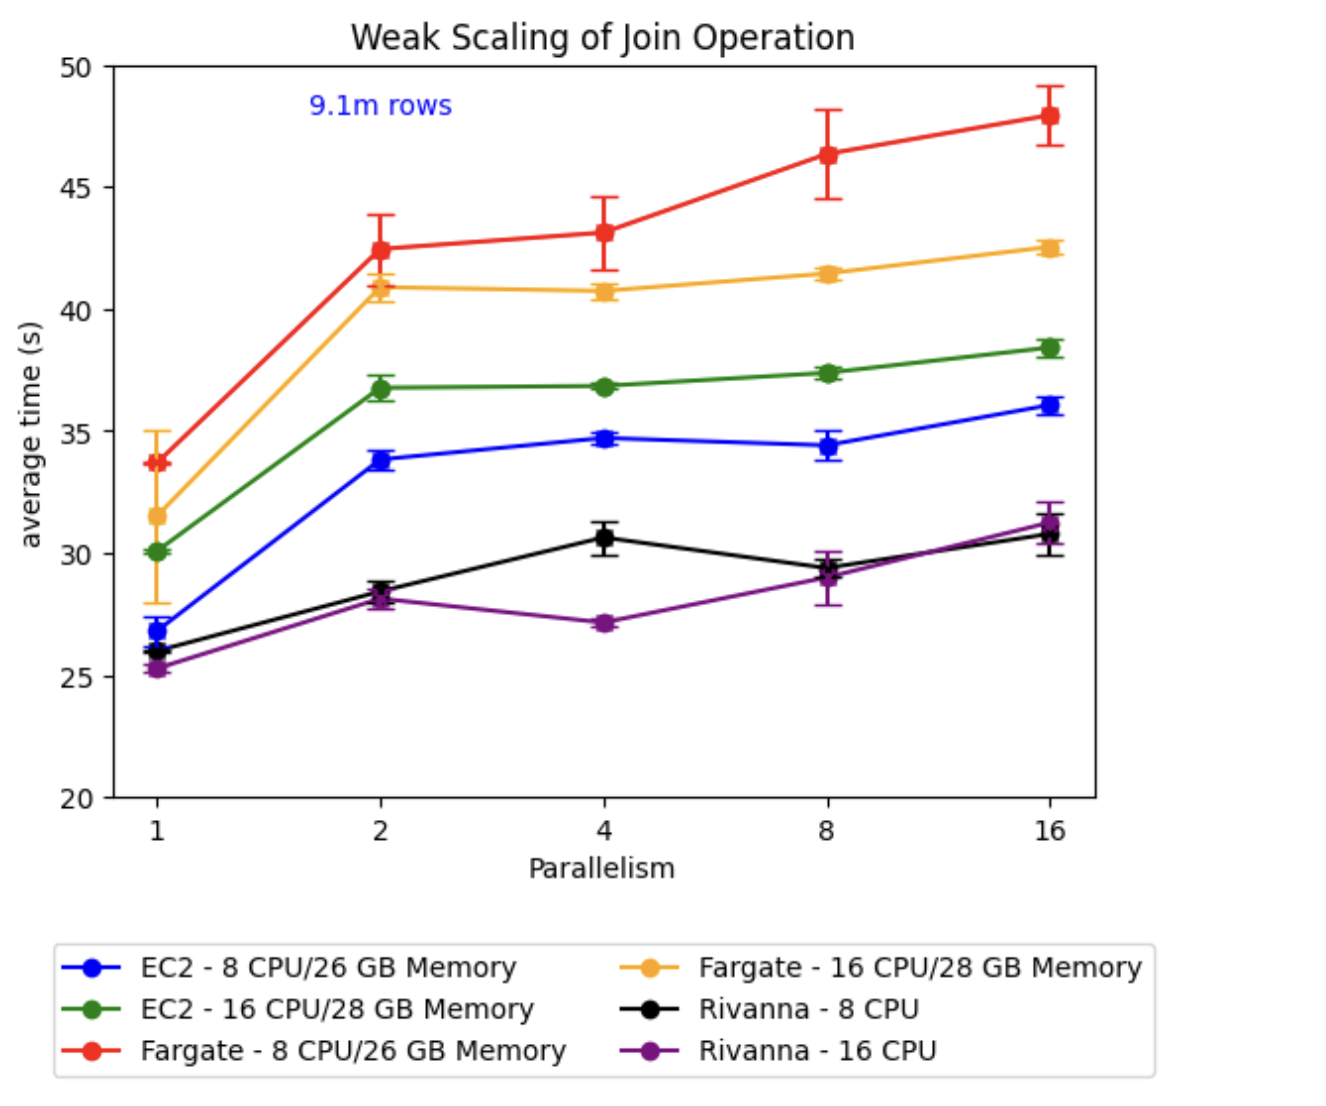
\includegraphics[width=\linewidth]{source/Figure/weakscaling1.png}
    \end{center}
    \caption{Comparison of weak scaling for the Join operation across infrastructure}
    \label{fig:weakscaling1}
\end{figure}

\begin{table}
%\setlength{\tabcolsep}{5pt}
	\centering
	\caption{Execution Time of Strong Scaling from Join Operations Across Infrastructure.}
	\label{tab:strong-exp_table}
	\begin{tabular}{llcr @{\hspace{1\tabcolsep}} lr @{\hspace{1\tabcolsep}} l}
		%
		\toprule
		                   &
		               &
		                     &
		\multicolumn{2}{c}{Execution Time}         \\
	    		%
		Infrastructure             &
		Scaling               &
		Parallelism                     &
		\multicolumn{2}{c}{time (seconds)}                    \\
		%
		\midrule
		\multirow{5}{*}{EC2 8 CPU/26 GB} &
		\multirow{5}{*}{strong} &
		1                       &
		495.40 & $\pm4.75$     \\
		%
		&
		                     &
		2                     &
		302.65 & $\pm2.77$   \\
		%
		&
		                   &
		4                     &
		142.43 & $\pm1.39$    \\
		%
		                    & &
		8                     &
		69.86 & $\pm1.08$      \\
  		%
		                    & &
		16                     &
		35.88 & $\pm0.46$      \\

        \cmidrule{2-5}
    	\multirow{5}{*}{EC2 16 CPU/28 GB} &
		\multirow{5}{*}{Strong} &
		1                       &
		535.91 & $\pm1.40$     \\
		%
		&
		                     &
		2                     &
		308.64 & $\pm2.64$   \\
		%
		&
		                   &
		4                     &
		156.23 & $\pm0.66$    \\
		%
		                    & &
		8                     &
		77.36 & $\pm0.27$      \\
  		%
		                    & &
		16                     &
		38.89 & $\pm0.52$      \\

		\cmidrule{2-5}
    	\multirow{5}{*}{Fargate 8 CPU/26 GB} &
		\multirow{5}{*}{Strong} &
		1                       &
		600.40 & $\pm1.42$     \\
		%
		&
		                     &
		2                     &
		370.67 & $\pm10.69$   \\
		%
		&
		                   &
		4                     &
		190.92 & $\pm7.27$    \\
		%
		                    & &
		8                     &
		92.44 & $\pm2.41$      \\
  		%
		                    & &
		16                     &
		47.68 & $\pm1.11$      \\
		
		\cmidrule{2-5}
    	\multirow{5}{*}{Fargate 16 CPU/28 GB} &
		\multirow{5}{*}{Strong} &
		1                       &
		589.65 & $\pm5.88$     \\
		%
		&
		                     &
		2                     &
		359.92 & $\pm0.76$   \\
		%
		&
		                   &
		4                     &
		173.39 & $\pm0.18$    \\
		%
		                    & &
		8                     &
		85.02 & $\pm0.04$      \\
  		%
		                    & &
		16                     &
		42.71 & $\pm0.0007$      \\

        \cmidrule{2-5}
    	\multirow{5}{*}{Rivanna 8 CPU} &
		\multirow{5}{*}{Strong} &
		1                       &
		328.02 & $\pm1.90$     \\
		%
		&
		                     &
		2                     &
		180.35 & $\pm0.91$   \\
		%
		&
		                   &
		4                     &
		120.38 & $\pm0.66$    \\
		%
		                    & &
		8                     &
		44.00 & $\pm0.61$      \\
  		%
		                    & &
		16                     &
		24.60 & $\pm1.97$      \\
        \cmidrule{2-5}
    	\multirow{5}{*}{Rivanna 16 CPU} &
		\multirow{5}{*}{Strong} &
		1                       &
		442.39 & $\pm1.67$     \\
		%
		&
		                     &
		2                     &
		242.31 & $\pm0.63$   \\
		%
		&
		                   &
		4                     &
		88.91 & $\pm1.03$    \\
		%
		                    & &
		8                     &
		43.80 & $\pm0.54$      \\
  		%
		                    & &
		16                     &
		31.62 & $\pm1.36$      \\
		\bottomrule
	\end{tabular}
\end{table}

Table \ref{tab:strong-exp_table} presents the results of strong scaling experiments involving 145 million rows.  Similar to weak scaling, we conduct the experiment four times, performing ten iterations for each trial.  The results of strong scaling are shown in Figure \ref{fig:strongscaling1}.  We observe high latencies across the infrastructure for fewer than four nodes, and a general convergence of latency as the number of nodes ranges from eight to sixteen.  This supports the validity of utilizing cloud resources as a viable alternative for data parallel preprocessing workloads.  We also assert that cost savings can be realized through cloud infrastructure, given the variable incremental costs compared to the fixed costs associated with traditional HPC clusters.


\begin{figure}[ht]
    \begin{center}
    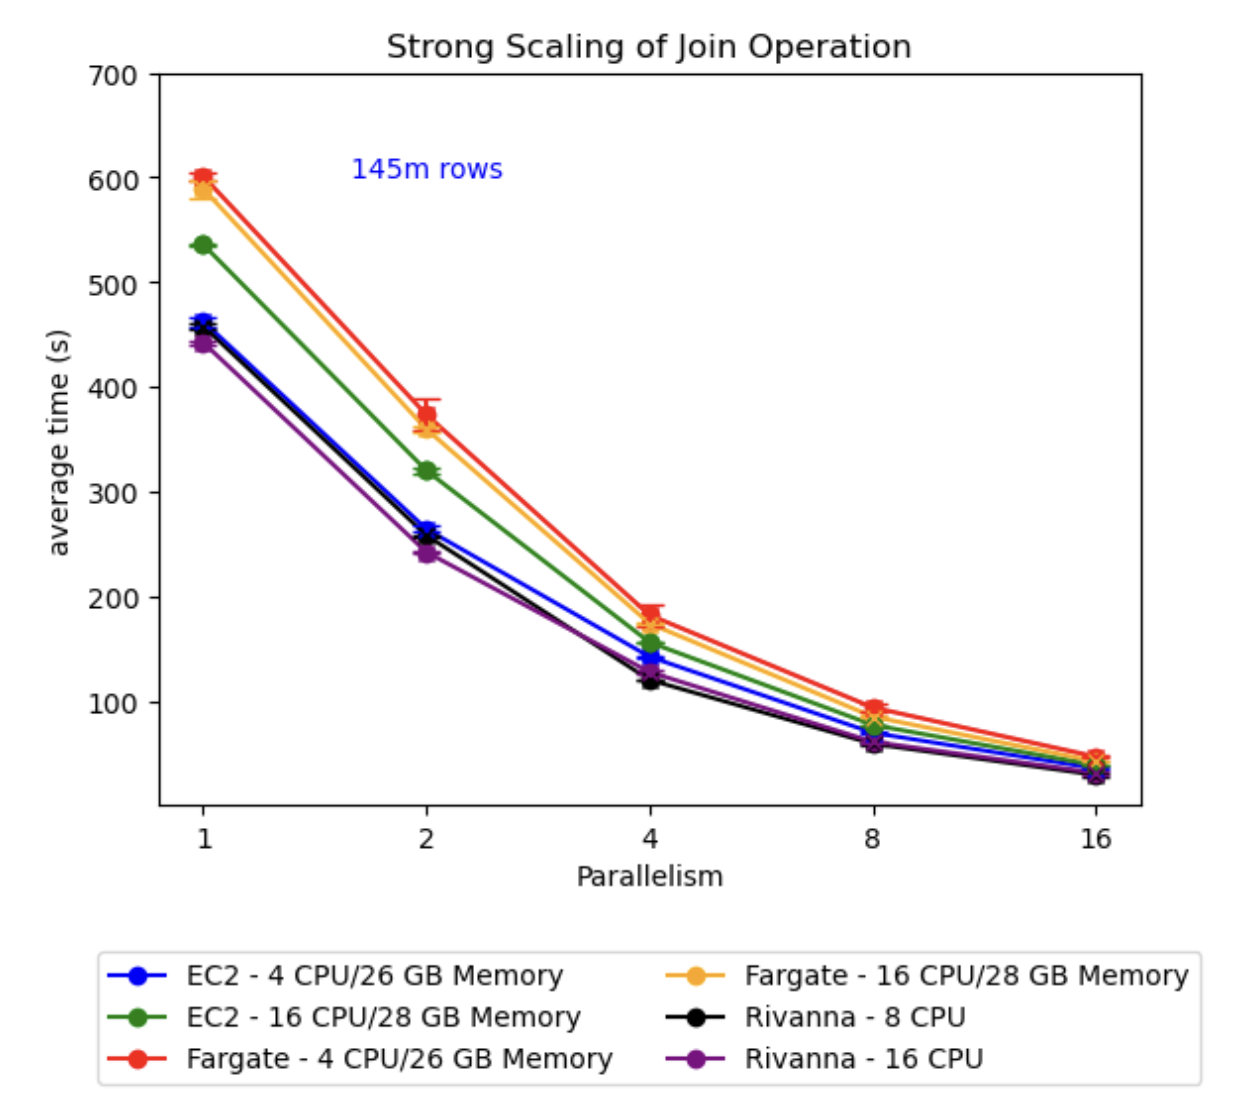
\includegraphics[width=\linewidth]{source/Figure/stongscal1.png}
    \end{center}
    \caption{Comparison of strong scaling for the Join operation across infrastructure}
    \label{fig:strongscaling1}
\end{figure}

We also conducted experiments on one node for AWS and Rivanna with 800000 rows to measure raw performance comparisons of CPUs on those systems.  The number of rows was selected based on memory availability on AWS T2 instances as the lowest common denominator.  We used EC2 (serverful) and Fargate (serverless) Containers on the AWS side.  For  EC2, we used T2 instances, one of the lowest-cost on-demand instance types.  T2 Nano instances (Intel(R) Xeon(R) CPU E5-2686 v4 @ 2.30GHz) were configured with one virtual CPU and .5 GB of memory available.  T2 Micro instances (Intel(R) Xeon(R) CPU E5-2676 v3 @ 2.40GHz) included one virtual CPU and 1 GB available memory.  For AWS Fargate, we used .5 and .25 CPU configurations with 1GB of memory available.  The underlying Fargate hosts used Intel(R) Xeon(R) Platinum 8259CL CPU @ 2.50GHz CPUs.  We executed a similar experiment for Rivanna using the standard partition with one core and one CPU.  Rivanna’s results appear to be three orders of magnitude faster than AWS entry-level instances, presumably based on the processing power of these containers based on the number of rows.  Based on other experiments, we can conclude that as the number of rows increases, Rivanna’s performance begins to converge with AWS weak scaling performance.  The Rivanna host CPU used an Intel(R) Xeon(R) Gold 6248 CPU @ 2.50GHz with forty cores and forty CPUs.  The results of this set of experiments are depicted in Figure \ref{fig:singlenode}.

\begin{figure}[ht]
    \begin{center}
    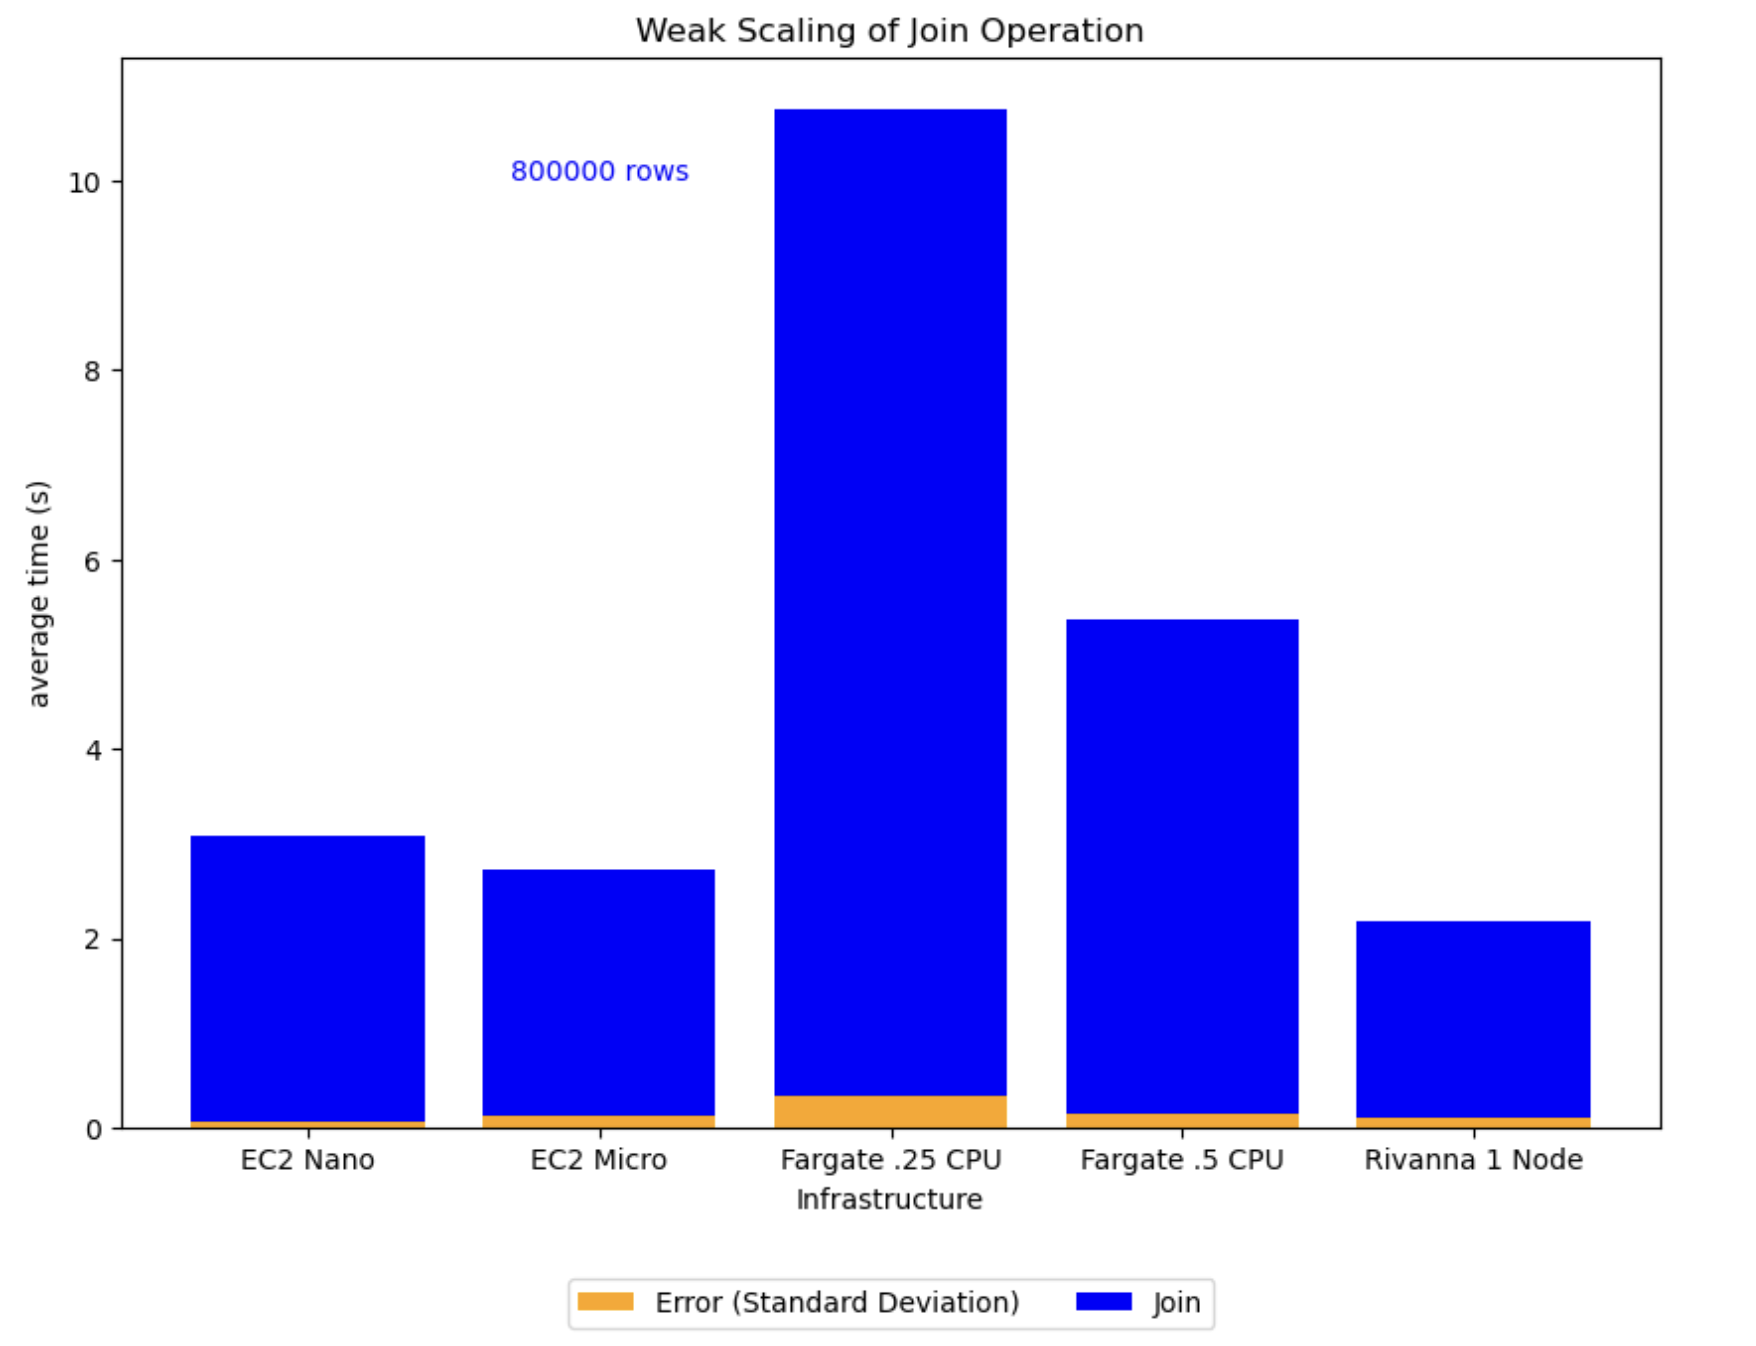
\includegraphics[width=\linewidth]{source/Figure/singleNodeExp.png}
    \end{center}
    \caption{Comparison of weak scaling for the Join operation across infrastructure for a Single Node}
    \label{fig:singlenode}
\end{figure}

For the last set of experiments, we ran scaling experiments plotted as speedup on AWS Lambda, EC2 ECS clusters and Rivanna.  Our intention was to run experiments on derivative configured infrastructure.  For EC2,  we used Ubuntu 22.04.2 LTS (Intel(R) Xeon(R) CPU E5-2670 v2 @ 2.50GHz) for hosts configured with two virtual CPU and 15 GB of memory (m3xlarge) and for hosts configured with one virtual CPU and 7.5 GB of memory (m3large).  For Rivanna, we ran experiments on 1 (standard partition) and 2, 4, 8, 16, 32 and 64 (parallel partition) CPU nodes (Intel(R) Xeon(R) Gold 6248 CPU @ 2.50GHz).  To match the performance and characteristics of AWS infrastructure on Rivanna, we configured experiments that would run on 10 and 6 GB memory configurations.  Rivanna experiments were executed in a Singularity container so that all experiments across infrastructure would be executed using dockerized processes.  For AWS Lambda, functions were configured to use 6GB and 10GB of memory.  Memory configuration influences the CPU available.  For the 6 GB configuration, 4 CPU cores are available, and for the 10 GB configuration, 6 CPU cores are available.  Both configurations use a custom-built AWS Lambda container that includes all the necessary Python and native libraries.  For weak scaling, we used 9.1 M rows, and for strong scaling, we used 4.5 million rows.  The choice of 4.5 million rows was necessary based on memory limitations imposed by AWS Lambda.  Note that additional executions on AWS Fargate (Serverless AWS ECS)  were intended, but changes were implemented by AWS that resulted in breaking the UCX transport discovery mechanism.  In the future, we plan to re-execute experiments using an updated configuration with the FMI library.

For these scaling experiments, we calculate speedup as the execution time ratio to the base case.  The base case is considered the slowest execution or the first node.  Speedup is defined as:
\[
    Speedup = \frac{\text{Baseline Time}}{\text{Parallel Time}}
\]

For the standard deviation or error propagation, we used the following formula applied to the observed standard deviation across executions (i.e., four separate experiments were completed for each node).

\[
    \frac{\Delta{S}}{S} = \sqrt{\left(\frac{\Delta{T_1}}{T_1}\right)^2 + \left(\frac{\Delta{T_2}}{T_2}\right)^2}
\]
\newline
Where:
\newline
\newline
S is the Speedup: S = $\frac{T_1}{T_2}$
\newline
\newline
$\Delta{S}$ is the error in speedup
\newline
\newline
$T_1$ is the baseline execution time (the time for one node)
\newline
\newline
$\Delta{T}_1$ is the error in baseline execution time
\newline
\newline
$T_2$ is the parallel execution time
\newline
\newline
$\Delta{T}_2$ is the error in parallel execution time
\newline
\newline
For these experiments, Figure \ref{fig:weakscalinground3} depicts the weak scaling results, and the strong scaling results are depicted in Figure \ref{fig:strongscalinground3}. 


\begin{figure}[ht]
    \begin{center}
    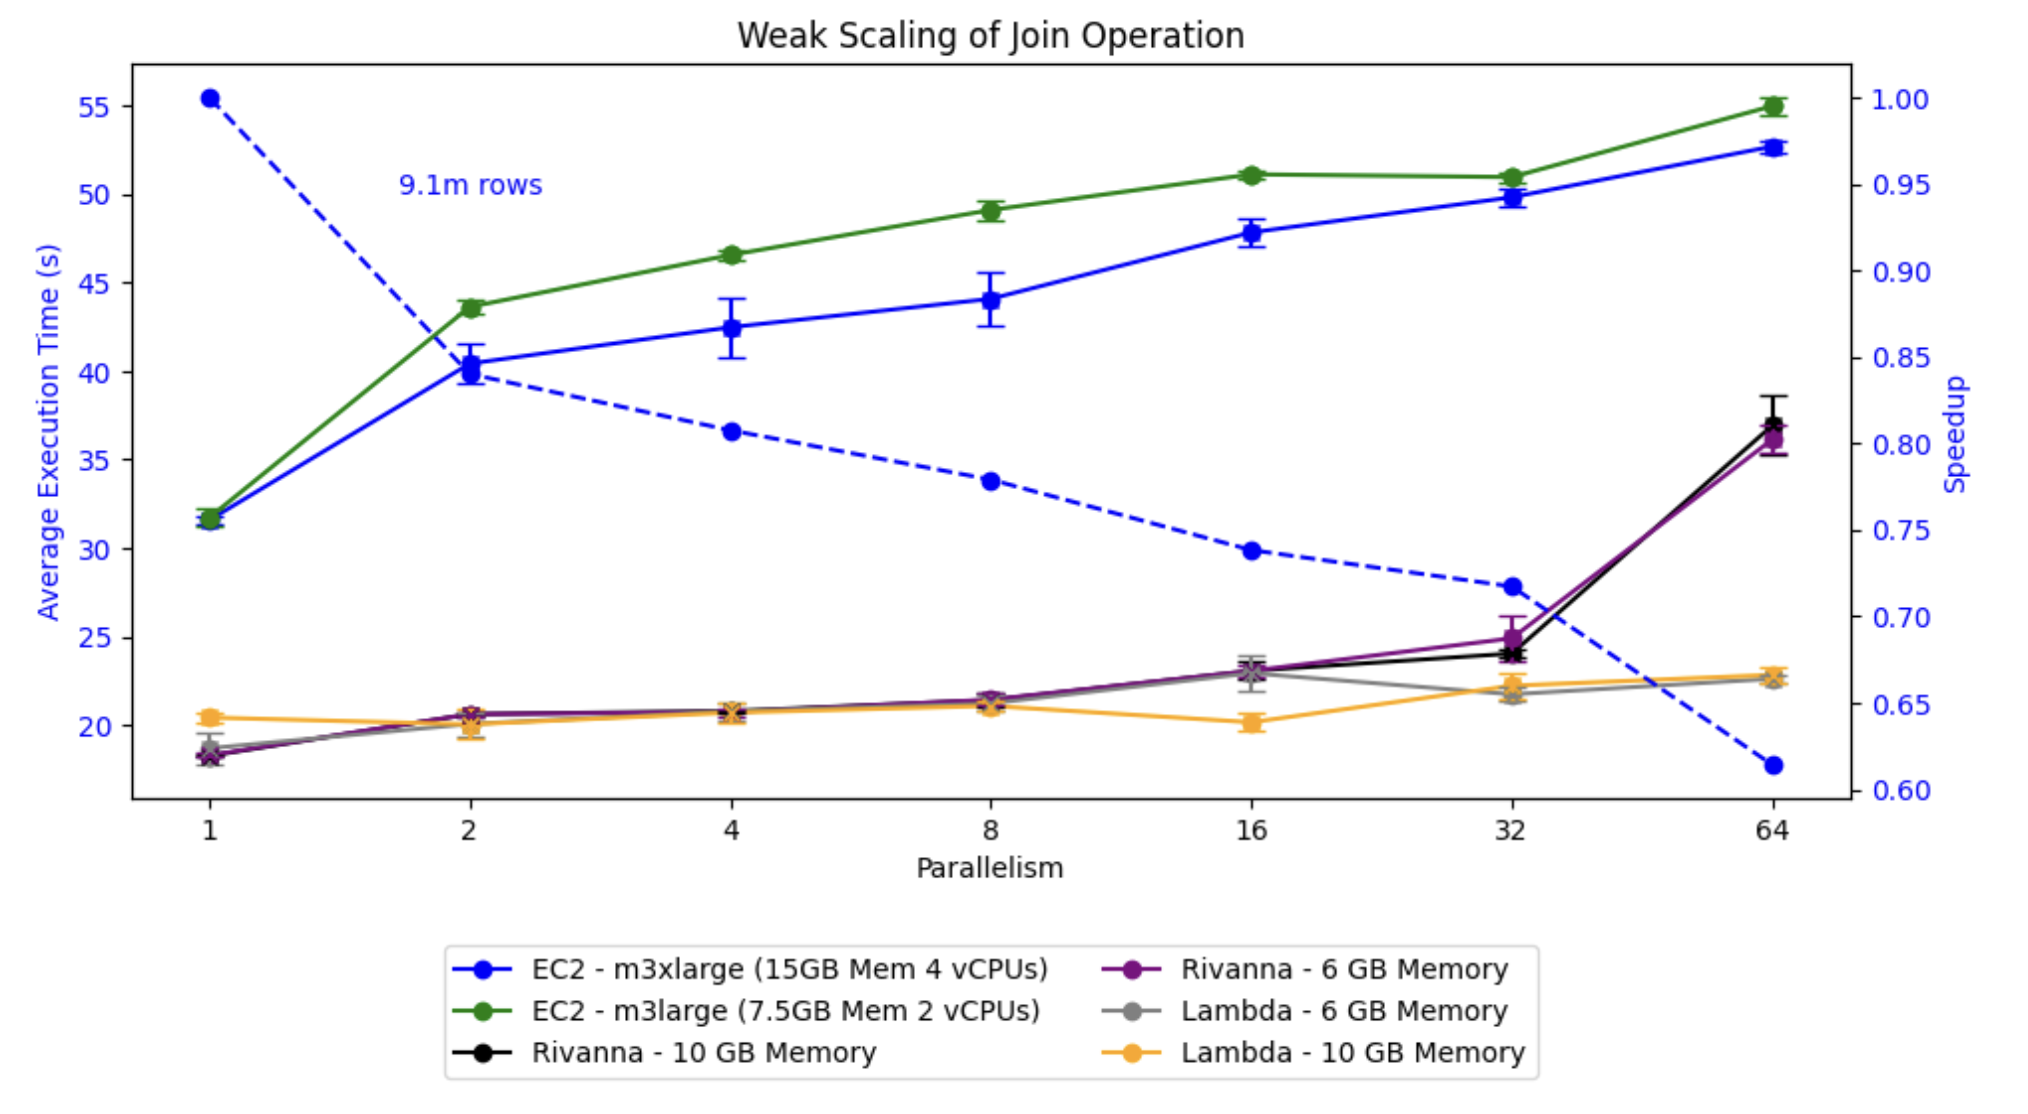
\includegraphics[width=\linewidth]{source/Figure/weekscalinground3.png}
    \end{center}
    \caption{Comparison of weak scaling for the Join operation across infrastructure including AWS Lambda}
    \label{fig:weakscalinground3}
\end{figure}

\begin{figure}[ht]
    \begin{center}
    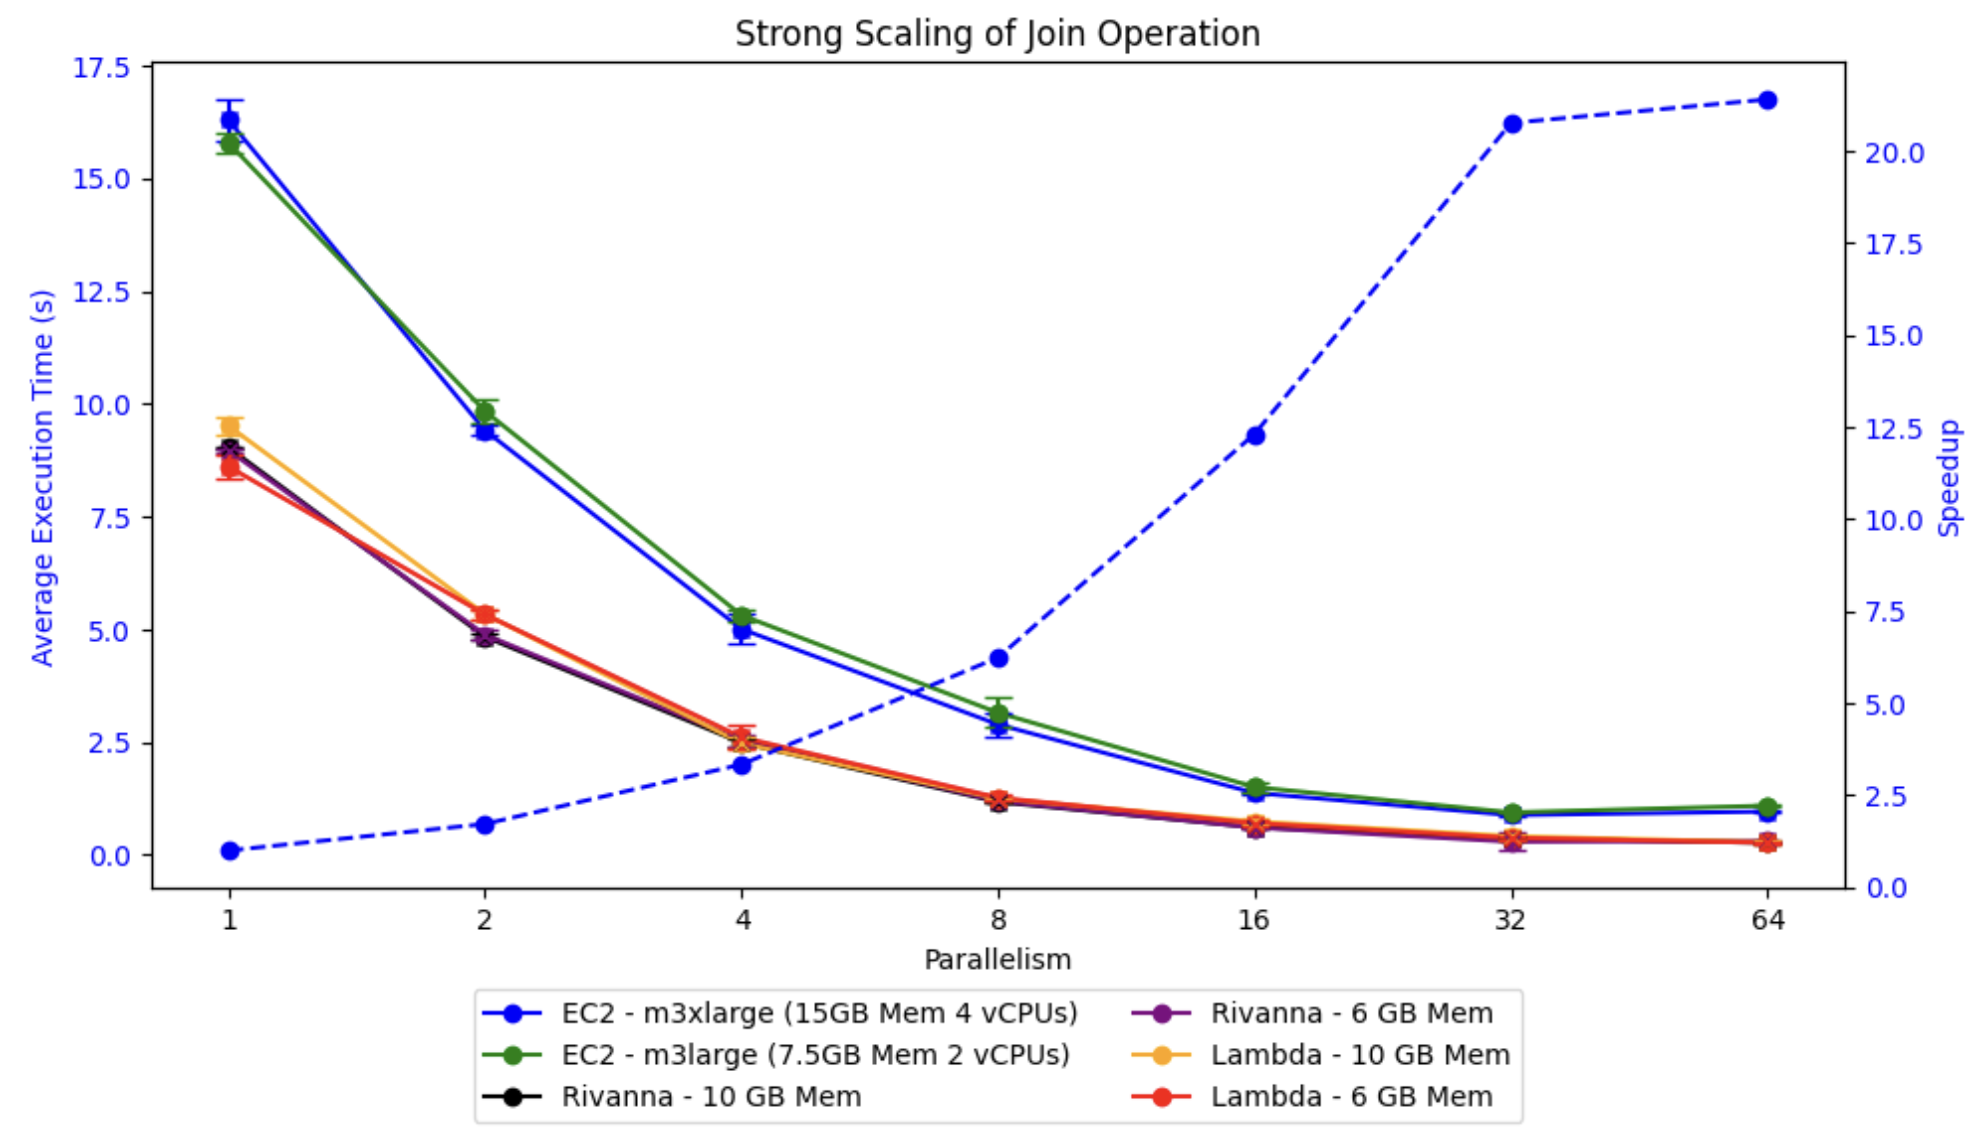
\includegraphics[width=\linewidth]{source/Figure/strongscalinground3.png}
    \end{center}
    \caption{Comparison of strong scaling for the Join operation across infrastructure including AWS Lambda}
    \label{fig:strongscalinground3}
\end{figure}